\documentclass{article}
\usepackage[utf8]{inputenc}
\usepackage{graphicx} % figuras
\usepackage{subfigure} % subfiguras
\title{Procesamiento de InSAR}
\author{Cecilia Gómez Jiménez}
\date{August 2019}

\begin{document}

\maketitle

\section{Manual de procesamiento}
\textbf{Abrir los datos con el Sentinel Toolbox}\\

En la interfaz del Sentinel Toolbox,es necesario dirigirse al menú de File y seleccionar Open Product.Se procede a seleccionar la carpeta que contiene el archivo de Sentinel-1 SLC ,seleccionando el archivo con formato .zip .\\
%%%%%%%%%%%%%%%%%%%%%%%%%%%%%%%%%%%%%
    \begin{figure}[htbp]
    \centering
    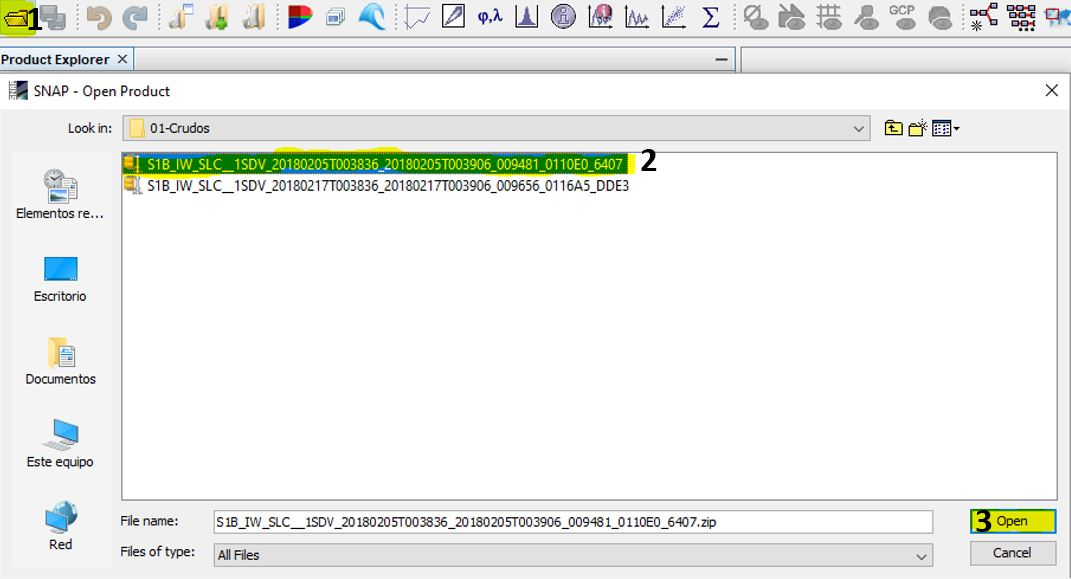
\includegraphics[width=8cm]{Imagen/02.JPG}
    \caption{Cargar datos.}
    \label{fig:01}
    \end{figure}\\
%%%%%%%%%%%%%%%%%%%%%%%%%%%%%%%%%%%%%
\textbf{Formato de los datos SLC}\\
La información relevante de la imagen se observa al desplegar la pestaña del archivo .zip .

\begin{itemize}
    \item Metadatos: parámetros relacionados con la órbita y los datos.
    \item Vector Data:Puede contener puntos de control y pins de lugares importantes.
    \item Cuadrículas “Tie Point”: interpolación de latitud/longitud, ángulo de incidencia etc.
    \item Quicklooks: Imagen la cual contiene los pases de escena en coordenadas de radar.
    \item Bandas: valores complejos para cada sub-barrido “i” y “q” e intensidad (la intensidad es la amplitud al cuadrado, una banda virtual).
\end{itemize}
    %%%%%%%%%%%%%%%%%%%%%%%%%%%%%%
    \begin{figure}[htbp]
    \centering
    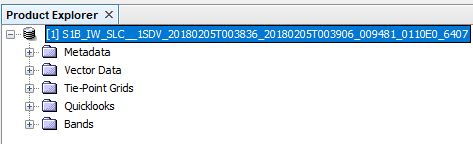
\includegraphics[width=8cm]{Imagen/01.JPG}
    \caption{Información relevante.}
    \label{fig:02}
    \end{figure}
    %%%%%%%%%%%%%%%%%%%%%%%%%%%%%%
\textbf{Preparación de Datos Interferométricos}\\

\begin{itemize}
    \item Co-rregistro de imágenes SAR
\end{itemize}
En el menú de la barra superior del software,SNAP, se busca la opción \textit{Radar},posteriormente \textit{Coregistration}, después \textit{S1 TOPS Coregistration}, y finalmente \textit{S1 TOPS Coregistration}, nuevamente.


%%%%%%%%%%%%%%%%%%%%%%%%%%%%%%%%%%%%%%%%
    %%%%%%%%%%%%%%%%%%%%%%%%%%%%%%
    \begin{figure}[htbp]
    \centering
    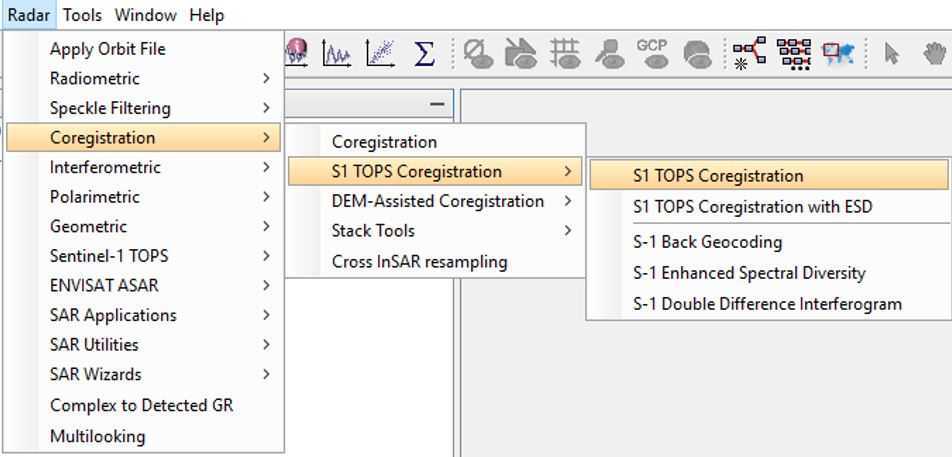
\includegraphics[width=8cm]{Imagen/03.JPG}
    \caption{Procesamiento Co-rregistro.}
    \label{fig:03}
    \end{figure}
    %%%%%%%%%%%%%%%%%%%%%%%%%%%%%%%%%%%%%%
    \begin{figure}[htbp]
    \centering
    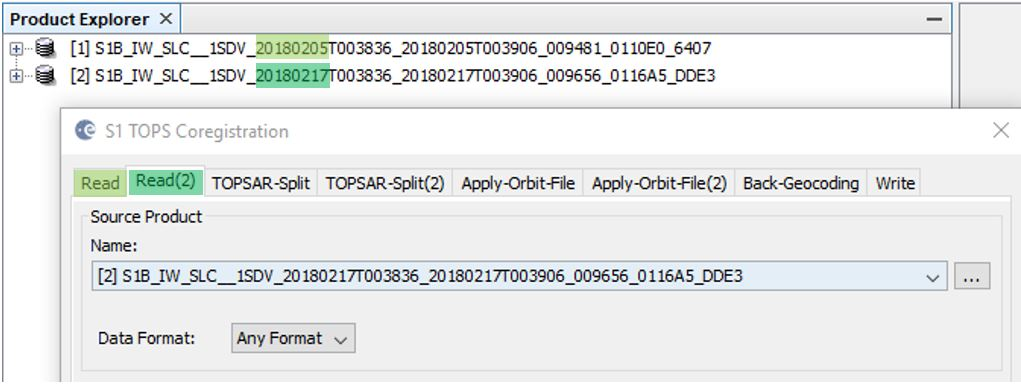
\includegraphics[width=8cm]{Imagen/04.JPG}
    \caption{Parámetros Read.}
    \label{fig:04}
    \end{figure}
    %%%%%%%%%%%%%%%%%%%%%%%%%%%%%%
    %%%%%%%%%%%%%%%%%%%%%%%%%%%%%%
    En la pestaña \textit{Read},se selecciona el archivo SLC con la temporalidad más lejana al día actual  y en la pestaña Read(2) se selecciona el archivo SLC con la temporalidad más cercana al día actual.\\ 
    %%%%%%%%%%%%%%%%%%%%%%%%%%%%%%
    En las pestañas \textit{TOPSAR-Split} y \textit{TOPSAR-Split(2)}, se selecciona el  Subswath(IW1,IW2 o IW3) y la Polarización \textit{VH o VV}.\\ 
    %%%%%%%%%%%%%%%%%%%%%%%%%%%%%
    En la pestaña \textit{Back-Geocoding}, se selecciona el modelo digítal de elevación a usar,la cual se descarga de forma automática durante el procesado.\\ 
        %%%%%%%%%%%%%%%%%%%%%%%%%%%%%%%%%%%%%%
    \begin{figure}[htbp]
    \centering
    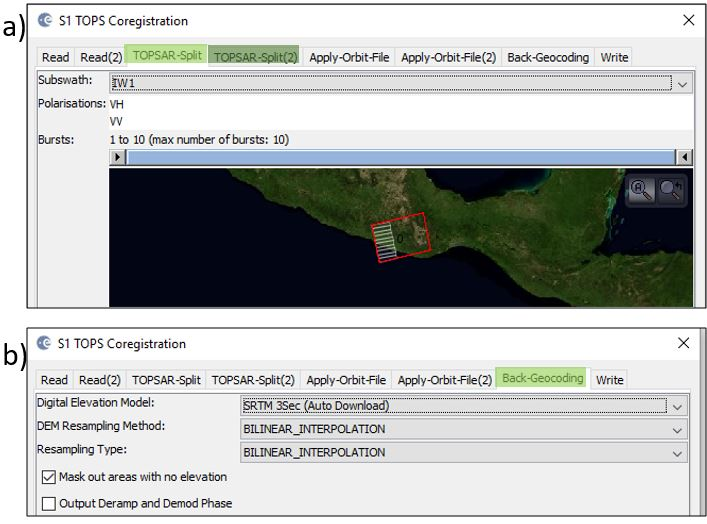
\includegraphics[width=8cm]{Imagen/05.JPG}
    \caption{a)Parámetros TOPSAR  b)Parámetros Back-Geocoding. }
    \label{fig:05}
    \end{figure}
    %%%%%%%%%%%%%%%%%%%%%%%%%%%%%%
    %%%%%%%%%%%%%%%%%%%%
    En la pestaña de \textit{Write}, se selecciona  la carpeta donde se guardan los resultados del procesamiento .\\ \\ \\
    %%%%%%%%%%%%%%%%%%%%
    %%%%%%%%%%%%%%%%%%%%%%%%%%%%%%
\textbf{Formando un Interferograma}\\
\begin{itemize}
    \item Procesamiento Interferométrico
\end{itemize}
    %%%%%%%%%%%%%%%%%%%%%%%%%%%%%%
    \begin{figure}[htbp]
    \centering
    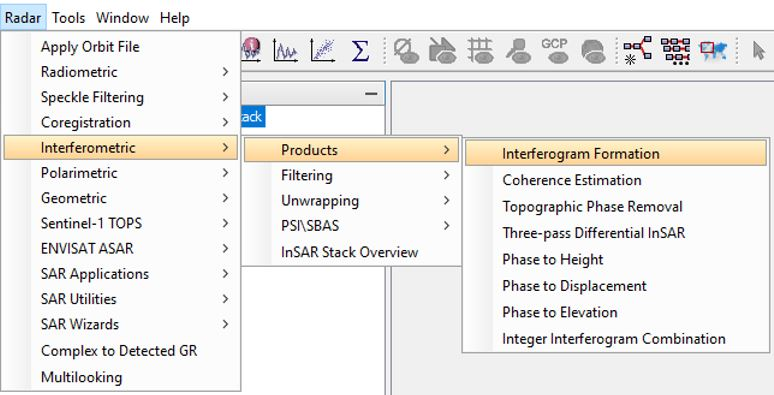
\includegraphics[width=9cm]{Imagen/06.JPG}
    \caption{Formación de un interferograma.}
    \label{fig:06}
    \end{figure}
    %%%%%%%%%%%%%%%%%%%%%%%%%%%%%%
    El segundo paso de la interferometría es hacer un interferograma a partir de las imágenes SLC co-registradas.\\
    En el menú de la barra superior, se selecciona \textit{Radar}, luego \textit{Interferometric}, posteriormente \textit{Products} y después \textit{Interferogram Formation}.\\
    En la pestaña \textit{I/O Parameters}, se selecciona el producto \textit{“Orb\_Stack”} creado por el paso anterior,  co-registro.    %%%%%%%%%%%%%%%%%%%%%%%%%%%%%%
\begin{figure}[htbp]
    \centering
    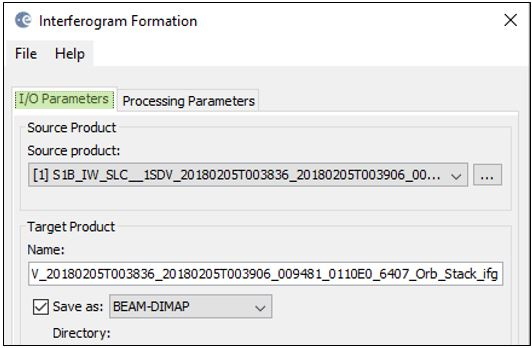
\includegraphics[width=9cm]{Imagen/07.JPG}
    \caption{Datos de entrada.}
    \label{fig:07}
    \end{figure}
    %%%%%%%%%%%%%%%%%%%%%%%%%%%%%%
    El archivo de salida después del procesamiento se coloca en la misma carpeta,,automáticamente y se le agrega “ifg” al nombre del archivo .
    Para un procesamiento básico, no hay necesidad de cambiar las configuraciones preprogramadas en la pestaña \textit{Processing Paramete}.\\ \\
    %%%%%%%%%%%%%%%%%%%%%%%%%%%%%%
    
\begin{itemize}
    \item Debursting TOPS
\end{itemize}
    El siguiente paso de la interferometría con datos de Sentinel-1 modo TOPS(IWS) es el “debursting” o el combinar las tomas (bursts). Esto no es necesario con datos de Sentinel-1 u otros stripmaps SAR.
    
    En el menú de la barra superior del software SNAP,se selecciona \textit{Radar}, luego \textit{Sentinel-1 TOPS}y después \textit{S-1 TOPS deburst}.
    
    En la pestaña \textit{I/O Parameters},se selecciona el producto \textit{I/O Parameters} “Orb \_Stack \_ifg” creado por el paso de formación del interferograma.Por defecto, al archivo de salida se le agrega “deb” al nombre.No es necesario cambiar la pestaña de \textit{Processing Parameters}.\\ \\ \\ \\ \\ \\
    %%%%%%%%%%%%%%%%%%%%%%%%%%%%%%
\begin{figure}[htbp]
\begin{minipage}[b]{0.5\linewidth}
\centering
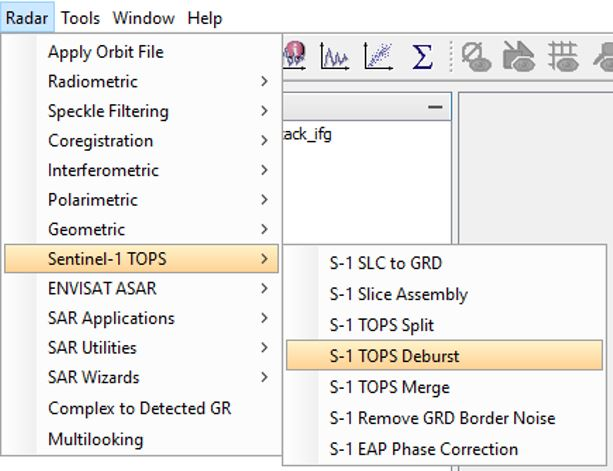
\includegraphics[width=\linewidth]{Imagen/08.JPG}
\caption{Acceder a la ventana de procesamiento Deburts.}
\label{fig:figura8}
\end{minipage}
\hspace{0.5cm}
\begin{minipage}[b]{0.5\linewidth}
\centering
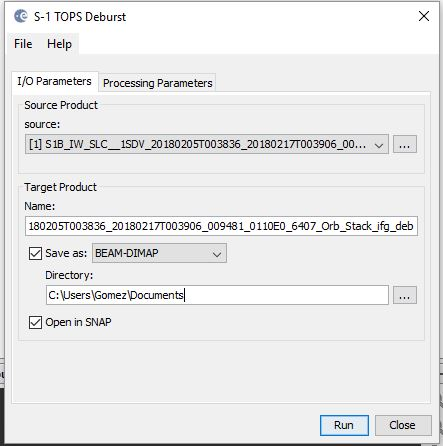
\includegraphics[width=\linewidth]{Imagen/09.JPG}
\caption{Ventana de procesamiento Deburts.}
\label{fig:figura9}
\end{minipage}
\end{figure}
    %%%%%%%%%%%%%%%%%%%%%%%%%%%%%%%%%%%%%5
\begin{itemize}
    \item Remoción de la Fase Topográfica
\end{itemize}    
     El siguiente paso para toda interferometría es
remover la fase topográfica mediante un DEM.

En el menú de la barra superior, se selecciona
\textit{Radar},luego \textit{Interferometric}, posteriormente \textit{Products} y finalmente \textit{Topographic Phase Removal} .Por defecto, al archivo de salida se le
agrega “dinsar” al nombre,en la pestaña \textit{Processing Parameters}se muestra que la configuración
preprogramada se descarga el \textit{SRTM 3 1Sec HGT}, el cual sirve para un preprocesamiento básico, pero puede
que necesite otro DEM en algunos casos.De acuerdo al foro STEP Forum también se puede usar \textit{SRTM 3 1Sec HGT} para un procesamiento básico.\\ \\ \\ \\ \\ \\ \\ \\ \\ \\ \\ \\ \\ \\ \\ \\ \\ \\ \\ \\ \\ \\ \\ \\ \\ \\ \\ \\ \\ \\ \\ \\ \\

%%%%%%%%%%%%%%%%%%%%%%%%%%%%%
 %%%%%%%%%%%%%%%%%%%%%%%%%%%%%%
\begin{figure}[htbp]
    \centering
    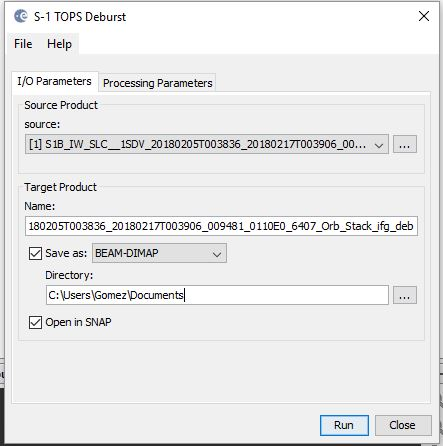
\includegraphics[width=9cm]{Imagen/09.JPG}
    \caption{Ventana de procesamiento Topographic Phase Removal.}
    \label{fig:07}
    \end{figure}
    %%%%%%%%%%%%%%%%%%%%%%%%%%%%%%
%%%%%%%%%%%%%%%%%%%%%%%%%%%%%
\begin{figure}[htbp]
\begin{minipage}[b]{0.5\linewidth}
\centering
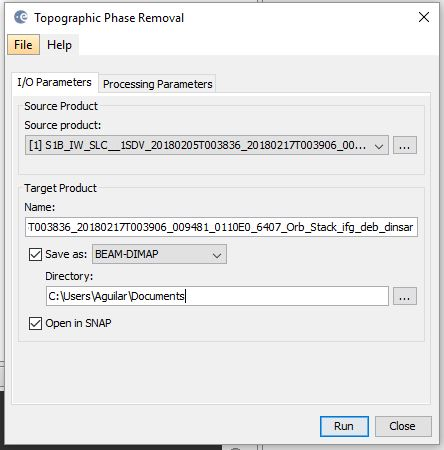
\includegraphics[width=\linewidth]{Imagen/10.JPG}
\caption{Acceder a la ventana de Remoción de la Fase Topográfica }
\label{fig:figura10}
\end{minipage}
\hspace{0.2cm}
\begin{minipage}[b]{0.5\linewidth}
\centering
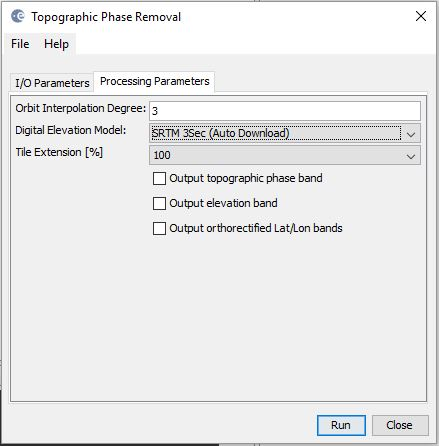
\includegraphics[width=\linewidth]{Imagen/11.JPG}
\caption{Datos de entrada y de salida de Topographic Phase Removal.}
\label{fig:figura11}
\end{minipage}
\hspace{0.2cm}
\begin{minipage}[b]{0.5\linewidth}
\centering
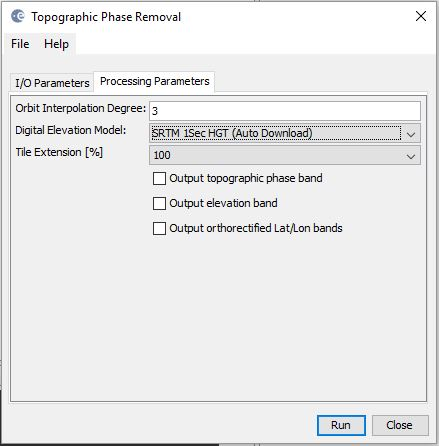
\includegraphics[width=\linewidth]{Imagen/12.JPG}
\caption{Ventana de procesamiento Topographic Phase Removal.}
\label{fig:figura12}
\end{minipage}
\end{figure}
%%%%%%%%%%%%%%%%%%%%%%%%%%%%%
Hay dos pasos que ayudan a reducir el nivel de ruido en un interferograma,el filtrado y multi-looking.El filtrado se aplicará en primera instancia, sin embargo también se puede hacer el multi-looking primero.
%%%%%%%%%%%%%%%%%%%%%%%%%%%%%
\begin{itemize}
    \item Filtrado 
\end{itemize} 
En el menú de la barra superior,se selecciona \textit{Radar}, luego \textit{Interferometric} ,posteriormente \textit{Filtering} , y después \textit{Goldstein Phase Filtering}.En la pestaña \textit{I/O Parameters} ,se selecciona el producto \textit{“dinsar”} creado en el paso anterior.Por defecto, al archivo de salida se le agrega \textit{“flt”} al nombre.Para un procesamiento básico, no hay necesidad de cambiar los valores
preprogramados en la pestaña \textit{Processing Parameters}.
%%%%%%%%%%%%%%%%%%%%%%%%%%%%%
    %%%%%%%%%%%%%%%%%%%%%%%%%%%%%%
\begin{figure}[htbp]
\begin{minipage}[b]{0.5\linewidth}
\centering
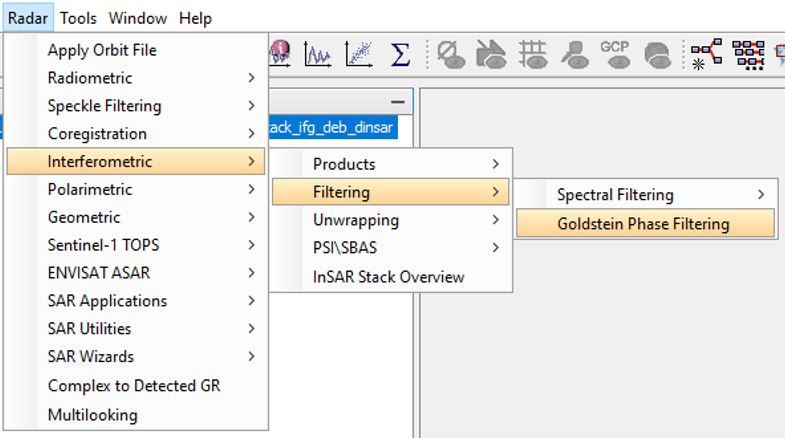
\includegraphics[width=\linewidth]{Imagen/13.JPG}
\caption{Acceder a la ventana de procesamiento Filtering.}
\label{fig:figura13}
\end{minipage}
\hspace{0.5cm}
\begin{minipage}[b]{0.5\linewidth}
\centering
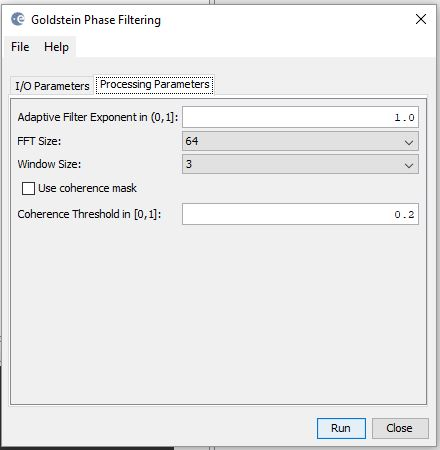
\includegraphics[width=\linewidth]{Imagen/14.JPG}
\caption{Ventana de procesamiento Filtering.}
\label{fig:figura14}
\end{minipage}
\end{figure}
    %%%%%%%%%%%%%%%%%%%%%%%%%%%%%%%%%%%%%5
%%%%%%%%%%%%%%%%%%%%%%%%%%%%%
\begin{itemize}
    \item Multi-Looking 
\end{itemize}
\textit{“Multi-looking”} significa sacarle el promedio a varios pixeles en cada dirección, se conoce como \textit{“darle varias miradas”} o varios \textit{“looks”}. El resultado son pixeles más
grandes y éstos pueden reducir la cantidad de ruidos de manera
significante. La cantidad de multi-looking que se debe hacer depende de la resolución espacial que uno necesita y el espaciamiento de las franjas.En el menú de la barra superior,se  selecciona \textit{Radar} y luego \textit{Multilooking}. En la pestaña \textit{I/O Parameters} , se selecciona el producto \textit{“dinsar\_flt”}  creado por el paso de filtrado y por defecto al archivo de salida se le agrega \textit{“ML”} al nombre.En la pestaña  \textit{Processing Parameters} ,se selecciona \textit{Source Bands}  \textit{“i\_ifg”,“q\_ifg”}  y \textit{“coh”} . Para esta escena, de ejemplo para ver como afecta el tamaño del pixel ,se escribe \textit{17 looks}  del rango y  calcula \textit{5 looks} en el azimut para producir  \backsim \textit{70 m} de pixeles de salida.Una aclaración importante es que no se debe elegir la banda  \textit{“Phase”},para finalmente dar en \textit{"Run"} y se realice el promedio.
%%%%%%%%%%%%%%%%%%%%%%%%%%%%
    %%%%%%%%%%%%%%%%%%%%%%%%%%%%%%
\begin{figure}[htbp]
\begin{minipage}[b]{0.3\linewidth}
\centering
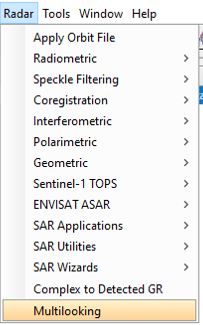
\includegraphics[width=\linewidth]{Imagen/15.JPG}
\caption{Acceder a la ventana de procesamiento Filtering.}
\label{fig:figura15}
\end{minipage}
\hspace{0.5cm}
\begin{minipage}[b]{0.5\linewidth}
\centering
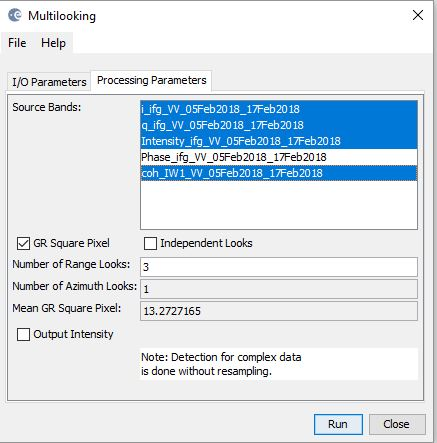
\includegraphics[width=\linewidth]{Imagen/16.JPG}
\caption{Ventana de procesamiento Filtering.}
\label{fig:figura16}
\end{minipage}
\end{figure}
    %%%%%%%%%%%%%%%%%%%%%%%%%%%%%%%%%%%%%5
     %%%%%%%%%%%%%%%%%%%%%%%%%%%%%%
\begin{figure}[htbp]
    \centering
    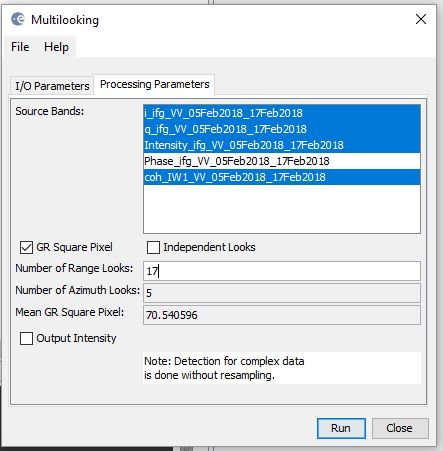
\includegraphics[width=9cm]{Imagen/17.JPG}
    \caption{Ventana de procesamiento Multilook.}
    \label{fig:07}
    \end{figure}
    %%%%%%%%%%%%%%%%%%%%%%%%%%%%%%
    Para poder Visualizar el  interferograma creado de Multi-Look, primero,se debe hacer una nueva banda de fase virtual después de realizar el “multi-looking” del interferograma complejo.En el menú de la barra superior de SNAP,se seleccione \textit{Raster}, después \textit{Data Conversion} y luego \textit{Complex i and q to Phase}.Finalmente se puede visualizar la nueva banda de fase.Cabe señalar que las franjas tienen mucho menos ruido. La relación de aspecto ha cambiado así que los pixeles son casi cuadrados en el suelo.La nueva imagen ahora mide 1207 pixeles transversalmente, mucho menos que los 20535 pixeles originales.
%%%%%%%%%%%%%%%%%%%%%%%%%%%%
\begin{itemize}
    \item Desenvolvimiento de Fase
\end{itemize}

\begin{enumerate}
	\item SNAP 6.0 no incluye desenvolvimiento de fase.\\ \\ Existe una forma de exportar el interferograma para desenvolverlo con el programa externo \textit{Snaphu (Statistical-cost,Network-flow Algorithm for Phase Unwrapping)} de Chen y Zebker.En el menú de la barra superior de SNAP,se selecciona \textit{Radar}, luego \textit{Interferometric} , después \textit{Unwrapping}  y finalmente \textit{Snaphu Export} .En la pestaña \textit{Read} , se selecciona el
producto \textit{“ML”} creado en el paso de \textit{multilooking} .En la pestaña \textit{Snaphu Export}, se puede cambiar el modo \textit{Statistical
-cost a “SMOOTH”} y el número de filas,columnas  y el numero de procesadores a “1” si no necesita realizar el promedio múltiple después del multi-looking. Se presiona  el botón \textit{Run}  y \textit{SNAP}  exporta la fase y coherencia del interferograma con un archivo \textit{“snaphu.conf”} 
        %%%%%%%%%%%
        %%%%%%%%%%%%%%%%%%%%%%%%%%%%%%
\begin{figure}[htbp]
\begin{minipage}[b]{0.6\linewidth}
\centering
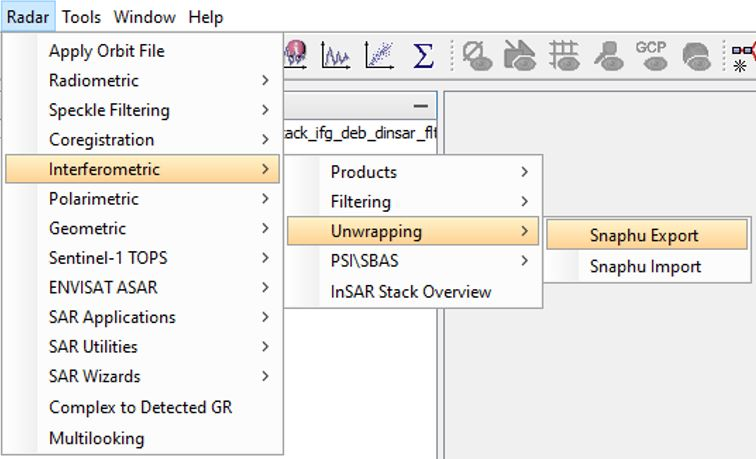
\includegraphics[width=\linewidth]{Imagen/22.JPG}
\caption{Acceder a la ventana de procesamiento Snaphu Export.}
\label{fig:figura22}
\end{minipage}
\hspace{0.5cm}
\begin{minipage}[b]{0.5\linewidth}
\centering
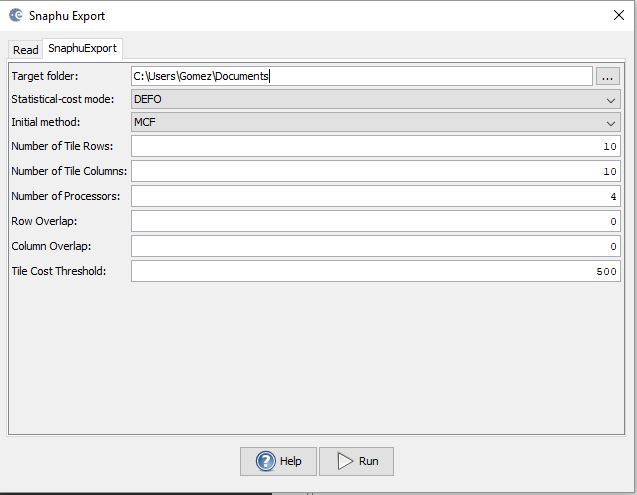
\includegraphics[width=\linewidth]{Imagen/23.JPG}
\caption{Ventana de procesamiento Standard Snaphu Export.}
\label{fig:figura23}
\end{minipage}
\hspace{0.5cm}
\begin{minipage}[b]{0.5\linewidth}
\centering
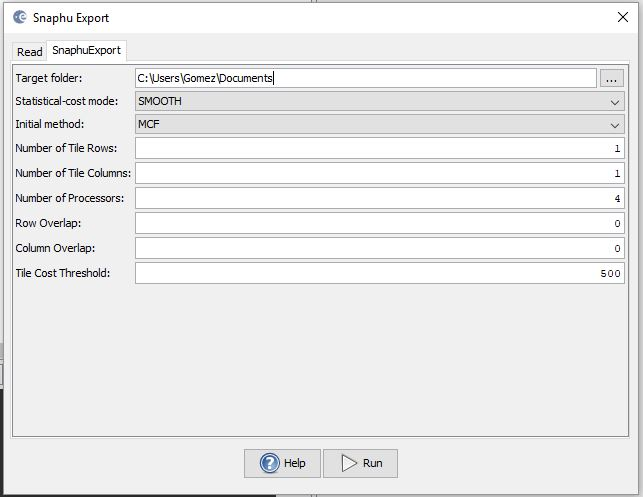
\includegraphics[width=\linewidth]{Imagen/24.JPG}
\caption{Ventana de procesamiento modificando el Standard Snaphu Export.}
\label{fig:figura24}
\end{minipage}
\end{figure}
    %%%%%%%%%%%%%%%%%%%%%%%%%%%%%%%%%%%%%5
        %%%%%%%%%%%
	%%%%%%%%%%%%%%%%%%%%%%%%%%%%%%%%%%%%%%
	\item Instalación de Snaphu\\ \\
ESA  ofrece ejecutables binarios prefabricados para sistemas de Windows de 32 o 64 bits en la página: http://step.esa.int/main/third-party-plugins- 2/snaphu/.Después del paso Snaphu Export en Snap,se debe ejecutar el programa Snaphu en la línea de comandos.Es necesario navegar a la carpeta “snaphu\_unw” y abrirla para poder ver la carpeta con el nombre del producto que exportó, por ejemplo,
S1B\_IW\_SLC\_1SDV\_20180205T00...Se necesita ir a esa carpeta.La carpeta debe contener la fase envuelta del interferograma \textit{“Phase\_ifg....img”} , la coherencia \textit{“coh\_*.img”}  y un archivo \textit{“snaphu.conf”} .El inicio del archivo \textit{“snaphu.conf”}muestra el comando Para ejecutar Snaphu, por ejemplo:

\# Command to call snaphu:\\ \\
\# \\ \\
\# snaphu -f snaphu.conf Phase\_ifg\_VV\_05Feb2018\_17Feb2018.snaphu
.img 1207  \\ \\

Puede que el programa Snaphu tarde en ejecutarse. Al final escribe la fase
desenvuelta en un archivo “Unw\_ifg*.img”
	%%%%%%%%%%%%%%%%%%%%%%%%%%%%%%%%%%%%%%
	\item  Importar la fase desenvuelta.
	%%%%%%%%%%%%%%%%%%%%%%%%%%%%%%%%%%%%%%
\end{enumerate}
En el menú de la barra superior de SNAP, se selecciona \textit{Radar} ,después \textit{Interferometric} , luego \textit{Unwrapping}  y finalmente \textit{Snaphu Import}.
La pestaña \textit{Read-Phase}  debe mostrar el producto envuelto que se exportó.En la pestaña \textit{Read-Unwrapped-Phase} ,se selecciona el producto fuente desenvuelto:Para ello es necesario navegar a la carpeta a la que se exportó Snaphu ,se selecciona el archivo \textit{“UnwPhase\_ifg...snaphu.hdr
”} .Es necesario ir a la pestaña \textit{Write}  y revisar el nombre del archivo de salida (se recomienda agregarle alguna palabra al final del nombre del producto envuelto y así se tiene un producto nuevo).
La fase desenvuelta sigue en radianes.La fase es la imagen de referencia
menos la imagen corregistrada. Si la imagen de referencia es anterior, la
fase negativa representa suelos en movimiento hacia el satélite (cambio
de rango negativo).
%%%%%%%%%%%%%%%%%%%%%%%%%%%%%%%%%%%%%%%
\begin{itemize}
    \item Conversión de Fase en Desplazamiento
\end{itemize}
Podemos convertir la fase desenvuelta en desplazamientos. En el menú de la barra superior de SNAP, se selecciona\textit{Radar}, luego \textit{Interferometric}, después \textit{Products}  y finalmente \textit{Phase to Displacement} .La pestaña \textit{I/O Parameters}  debe contener el producto desenvuelto que se importó ,el cual por defecto, se le agrega \textit{“\_dsp”}  al nombre del archivo objetivo.El desplazamiento está en metros.El signo cambió así que el desplazamiento positivo es “arriba” hacia el satélite en la dirección de la línea visual.
    %%%%%%%%%%%%%%%%%%%%%%%%%%%%%%
    %%%%%%%%%%%%%%%%%%%%%%%%%%%%%%
\begin{figure}[htbp]
\begin{minipage}[b]{0.6\linewidth}
\centering
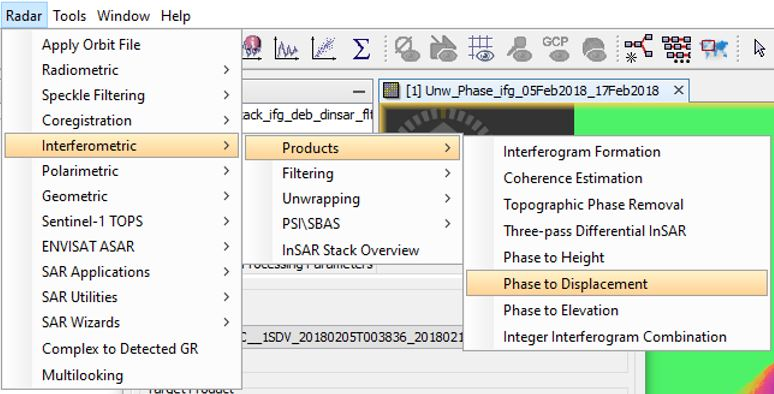
\includegraphics[width=\linewidth]{Imagen/19.JPG}
\caption{Acceder a la ventana de Phase to Displacement.}
\label{fig:figura19}
\end{minipage}
\hspace{0.5cm}
\begin{minipage}[b]{0.5\linewidth}
\centering
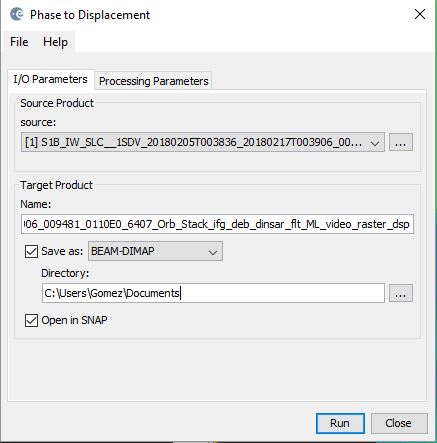
\includegraphics[width=\linewidth]{Imagen/18.JPG}
\caption{Ventana de procesamiento Phase to Displacement.}
\label{fig:figura18}
\end{minipage}
\end{figure}
    %%%%%%%%%%%%%%%%%%%%%%%%%%%%%%%%%%%%%5

\begin{itemize}
    \item Resultados de geocodificación—Corrección por Topografía
\end{itemize}
SNAP llama a la geocodificación con topografía \textit{“Terrain Correction”}. En el menú de la barra superior de SNAP,se selecciona \textit{Radar} , luego \textit{Geometric}, después \textit{Terrain Correction} , y finalmente \textit{Range Doppler Terrain Correction} .La pestaña \textit{I/O Parameters}  debe contener el producto de desplazamiento que importó (o algún otro de los productos ML).Por defecto se le agrega \textit{“\_TC”} al nombre del  objetivo.     %%%%%%%%%%%%%%%%%%%%%%%%%%%%%%
\begin{figure}[htbp]
\begin{minipage}[b]{0.6\linewidth}
\centering
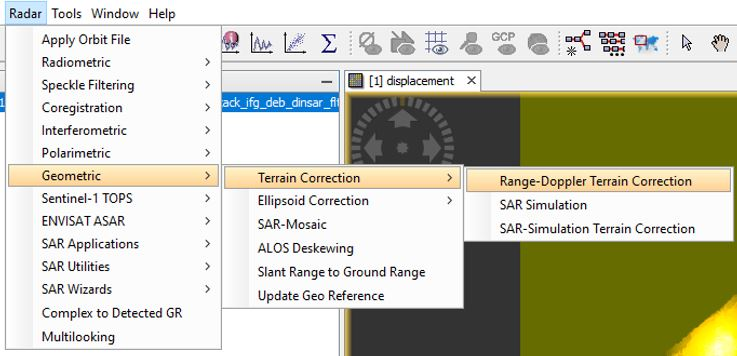
\includegraphics[width=\linewidth]{Imagen/20.JPG}
\caption{Acceder a la ventana de Range Doppler Terrain Correction.}
\label{fig:figura20}
\end{minipage}
\hspace{0.5cm}
\begin{minipage}[b]{0.4\linewidth}
\centering
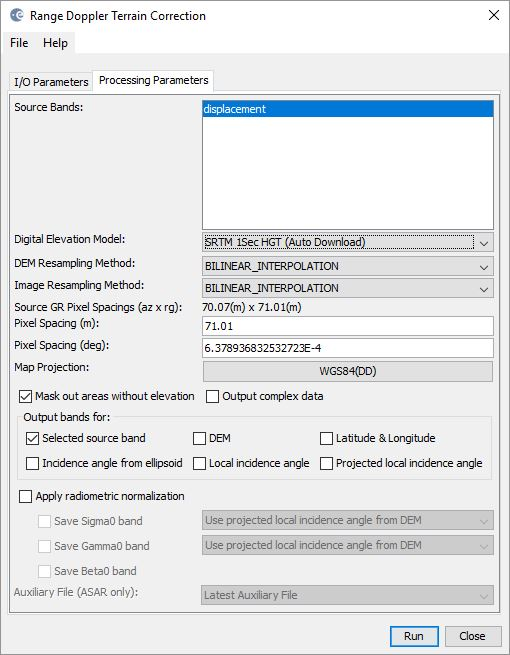
\includegraphics[width=\linewidth]{Imagen/21.JPG}
\caption{Ventana de procesamiento Range Doppler Terrain Correction.}
\label{fig:figura21}
\end{minipage}
\end{figure}
    %%%%%%%%%%%%%%%%%%%%%%%%%%%%%%%%%%%%%5
    \begin{itemize}
    \item Exportando el Mapa de Desplazamiento
    \end{itemize}
    
    Se puede exportar el mapa de desplazamiento geocodificado con la función \textit{File>Export} ,para un análisis con GIS, el formato \textit{GeoTIFF}  normalmente funciona bien.En QGIS, se puede usar \textit{”Add Raster Layer”} para leer el archivo \textit{GeoTIFF} .
    %%%%%%%%%%%%%%%%%%%%%%%
    \begin{itemize}
        \item Bibliografía
    \end{itemize}
    
    https://arset.gsfc.nasa.gov/sites/default/files/water/Brazil_2017/Day2/S4P1-span.pdf \\ \\
    
    https://arset.gsfc.nasa.gov/sites/default/files/disasters/Adv-SAR/SAR_S4-spanish.pdf
    


\end{document}